\documentclass{article}
\usepackage[spanish]{babel}
\usepackage[utf8]{inputenc}
\usepackage{graphicx}
\usepackage{minted}
\usepackage{courier}
\usepackage[dvipsnames]{xcolor}
\usepackage{relsize}
\usepackage{amsmath}
\usepackage{titlesec}

\definecolor{red}{rgb}{0.95,0.12,0.14}
\definecolor{green}{rgb}{0.47,0.58,0.17}
\definecolor{darkTurquoise}{rgb}{0.18,0.65,0.74}
\definecolor{blue}{rgb}{0.16,0,0.98}
\definecolor{purple}{rgb}{0.65,0.03,0.69}
\setlength\fboxsep{0pt}

\title{\textbf{Transacciones en Bitcoin}}
\author{Javier Domínguez Gómez \\
\small{jdg@member.fsf.org} \\
\small{Fingerprint: 94AD 19F4 9005 EEB2 3384 C20F 5BDC C668 D664 8E2B}}
\date{v0.1.03 - Junio 2019}

\begin{document}
\maketitle

\tableofcontents{}

\vspace{19mm}

\section{Introducción}
    \subsection{Formatos en el texto}
    A lo largo de este documento el lector encontrará algunas palabras o bloques de texto con diferentes formatos o tipografía. Se mostrarán en letra \textit{cursiva} las palabras en inglés o que hagan referencia a algún término técnico. Resaltadas o en \textbf{negrita} aquellas palabras que describen una propiedad, una variable o un nombre de fichero, y finalmente con tipografía \texttt{Courier} aquellos datos que representen un valor hexadecimal o base 16, o fragmentos de código fuente en diferentes lenguajes de programación.
    
    \subsection{Objetivo}
    Este documento presenta en detalle el la estructura de datos, composición, funcionamiento y tipos de las transacciones en el protocolo \textit{Bitcoin}\footnote{https://bitcoin.org/bitcoin.pdf}, además el lector podrá encontrar información acerca del lenguaje \textit{Bitcoin Script} que se emplea para el desarrollo e inclusión de programas llamados \textit{scripts} en las transacciones. Puesto que las transacciones son el elemento base donde ubicar los \textit{scripts} es necesario realizar un análisis forense a bajo nivel sobre cada una de las partes de las que se componen dentro del criptosistema definido por el protocolo \textit{Bitcoin}. Todos los datos utilizados en los ejemplos, así como en los cálculos, son datos reales pertenecientes al bloque número \texttt{\#}286819 de la cadena de bloques de \textit{Bitcoin} en la red principal \textit{mainnet}. No existe ninguna razón especial en la elección de este bloque, es uno al azar. El lector puede consultar los datos de este o cualquier otro bloque, bien en la cadena de bloques descargada en su computadora local o bien en un \textit{explorador de bloques online}\footnote{https://www.blockchain.com/en/btc/block-height/286819}, y realizar los mismos cálculos en todos los casos, obviamente obteniendo resultados diferentes.
    
    \subsection{A quién va dirigido}
    El documento va dirigido a principalmente a lectores que quieren desarrollar programas en lenguaje \textit{Bitcoin Script} para posteriormente utilizarlos como \textit{Smart Contracts} en la red del protocolo \textit{Bitcoin}. También va dirigido a lectores familiarizados con la criptología en cualquiera de sus dos ramas: la criptografía y el criptoanálisis, o a estudiantes de ciencias de la computación o matemáticas, en general a lectores que todavía no se han adentrado en el campo de del análisis forense sobre la información que contienelas transacciones de la cadena de bloques de \textit{Bitcoin}, pero que quieren comprender su funcionamiento al más bajo nivel, a nivel de \textit{bits}. El texto trata de facilitar al lector la información sobre los métodos empleados para poder identificar las transacciones dentro de un bloque de datos de \textit{Bitcoin}. Para ello será necesario tener de antemano unos conocimientos mínimos sobre conversión de datos en diferentes bases como decimal y hexadecimal.

\section{Datos de un bloque}
\begin{figure}[H]
\scriptsize{\texttt{$\sim$/.bitcoin/blocks/\$ hexdump\ -C\ -s\ 93725126\ -n\ 288\ blk00116.dat}}
    
    \scriptsize{
    \texttt{059621c6  \textbf{\textcolor{red}{f9 be b4 d9} \textcolor{green}{bd 53 02 00}  \textcolor{darkTurquoise}{02 00 00 00 17 97 5b 97}}  |.....S........[.|} \\
    \texttt{059621d6  \textbf{\textcolor{darkTurquoise}{c1 8e d1 f7 e2 55 ad f2  97 59 9b 55 33 0e da b8}}  |.....U...Y.U3...|} \\
    \texttt{059621e6  \textbf{\textcolor{darkTurquoise}{78 03 c8 17 01 00 00 00  00 00 00 00 8a 97 29 5a}}  |x.............)Z|} \\
    \texttt{059621f6  \textbf{\textcolor{darkTurquoise}{27 47 b4 f1 a0 b3 94 8d  f3 99 03 44 c0 e1 9f a6}}  |'G.........D....|} \\
    \texttt{05962206  \textbf{\textcolor{darkTurquoise}{b2 b9 2b 3a 19 c8 e6 ba  dc 14 17 87 35 8b 05 53}}  |..+:........5..S|} \\
    \texttt{05962216  \textbf{\textcolor{darkTurquoise}{53 5f 01 19 48 75 08 33}  \textcolor{blue}{63} \textcolor{purple}{01 00 00 00 01 00 00}}  |S\_..Hu.3c.......|} \\
    \texttt{05962226 \textbf{\textcolor{purple}{00 00 00 00 00 00 00 00  00 00 00 00 00 00 00 00}} |................|} \\
    \texttt{05962236 \textbf{\textcolor{purple}{00 00 00 00 00 00 00 00  00 00 00 00 00 00 ff ff}} |................|} \\
    \texttt{05962246 \textbf{\textcolor{purple}{ff ff 60 03 63 60 04 06  2f 50 32 53 48 2f 04 35}} |..`.c`../P2SH/.5|} \\
    \texttt{05962256 \textbf{\textcolor{purple}{8b 05 53 08 44 04 f2 53  00 00 17 e4 46 52 2c fa}} |..S.D..S....FR,.|} \\
    \texttt{05962266 \textbf{\textcolor{purple}{be 6d 6d 69 06 88 fb 88  6c 0d f0 c8 7c bc 7e a4}} |.mmi....l...|.~.|} \\
    \texttt{05962276 \textbf{\textcolor{purple}{f7 f1 b5 c0 05 0b d0 ac  37 51 cf c9 97 d9 d6 97}} |........7Q......|} \\
    \texttt{05962286 \textbf{\textcolor{purple}{13 28 de 04 00 00 00 00  00 00 00 48 61 70 70 79}} |.(.........Happy|} \\
    \texttt{05962296 \textbf{\textcolor{purple}{20 4e 59 21 20 59 6f 75  72 73 20 47 48 61 73 68}} | NY! Yours GHash|} \\
    \texttt{059622a6 \textbf{\textcolor{purple}{2e 49 4f 00 00 00 00 01  cb 81 31 95 00 00 00 00}} |.IO.......1.....|} \\
    \texttt{059622b6 \textbf{\textcolor{purple}{19 76 a9 14 80 ad 90 d4  03 58 1f a3 bf 46 08 6a}} |.v.......X...F.j|} \\
    \texttt{059622c6 \textbf{\textcolor{purple}{91 b2 d9 d4 12 5d b6 c1  88 ac 00 00 00 00 01 00}} |.....]..........|} \\
    \texttt{059622d6 \textbf{\textcolor{purple}{00 00 01 7d 67 7c de 17  3f 8c bf 43 31 27 a8 5e}} |...\}g|..?..C1'.\textasciicircum|
    \texttt{059622e6} ...}
    }
    \end{figure}

\section{Transacción \textit{Coinbase}}
    En el protocolo Bitcoin todos los bloques de la cadena de bloques contienen la misma estructura de datos para almacenar la información segmentada y ordenada en diferentes partes. La transacción \textit{Coinbase} es la primera transacción de cada bloque, es un espacio reservado para almacenar información relativa a la recompensa final por minar el bloque candidato y toda la información sobre comisiones adicionales en cada una de las transacciones que conformarán finalmente el bloque. Siguiendo con el ejemplo del bloque \texttt{\#}286819, podremos encontrar el inicio de la transacción \textit{Coinbase} a partir del \textit{byte} número 93.725.215, en el \textit{offset} \texttt{0x0596221f}, y en este caso abarca los siguientes 181 \textit{bytes} tal y como se muestra a continuación.
    \begin{figure}[H]
    \scriptsize{\texttt{$\sim$/.bitcoin/blocks/\$ hexdump\ -C\ -s\ 93725215\ -n\ 181\ blk00116.dat}}
        
        \scriptsize{
        \texttt{0596221f \textbf{\textcolor{purple}{01 00 00 00 01 00 00 00  00 00 00 00 00 00 00 00}} |................|} \\
        \texttt{0596222f \textbf{\textcolor{purple}{00 00 00 00 00 00 00 00  00 00 00 00 00 00 00 00}} |................|} \\
        \texttt{0596223f \textbf{\textcolor{purple}{00 00 00 00 00 ff ff ff  ff 60 03 63 60 04 06 2f}} |.........`.c`../|} \\
        \texttt{0596224f \textbf{\textcolor{purple}{50 32 53 48 2f 04 35 8b  05 53 08 44 04 f2 53 00}} |P2SH/.5..S.D..S.|} \\
        \texttt{0596225f \textbf{\textcolor{purple}{00 17 e4 46 52 2c fa be  6d 6d 69 06 88 fb 88 6c}} |...FR,..mmi....l|} \\
        \texttt{0596226f \textbf{\textcolor{purple}{0d f0 c8 7c bc 7e a4 f7  f1 b5 c0 05 0b d0 ac 37}} |...|.~.........7|} \\
        \texttt{0596227f \textbf{\textcolor{purple}{51 cf c9 97 d9 d6 97 13  28 de 04 00 00 00 00 00}} |Q.......(.......|} \\
        \texttt{0596228f \textbf{\textcolor{purple}{00 00 48 61 70 70 79 20  4e 59 21 20 59 6f 75 72}} |..Happy NY! Your|} \\
        \texttt{0596229f \textbf{\textcolor{purple}{73 20 47 48 61 73 68 2e  49 4f 00 00 00 00 01 cb}} |s GHash.IO......|} \\
        \texttt{059622af \textbf{\textcolor{purple}{81 31 95 00 00 00 00 19  76 a9 14 80 ad 90 d4 03}} |.1......v.......|} \\
        \texttt{059622bf \textbf{\textcolor{purple}{58 1f a3 bf 46 08 6a 91  b2 d9 d4 12 5d b6 c1 88}} |X...F.j.....]...|} \\
        \texttt{059622cf \textbf{\textcolor{purple}{ac 00 00 00 00 \ \ \ \ \ \ \ \ \ \ \ \ \ \ \ \ \ \ \ \ \ \ \ \ \ \ \ \ \ \ \ \ }} |.....|}}
    \end{figure}
    
    Otra manera de visualizar los datos de una transacción es mostrar todos los \textit{bytes} concatenados, sin espacios:
    
    \begin{figure}[H]
        \texttt{0x0100000001000000000000000000000000000000000000000000000} \\
        \texttt{0000000000000000000ffffffff6003636004062f503253482f04358b} \\
        \texttt{0553084404f253000017e446522cfabe6d6d690688fb886c0df0c87cb} \\
        \texttt{c7ea4f7f1b5c0050bd0ac3751cfc997d9d6971328de04000000000000} \\
        \texttt{004861707079204e592120596f7572732047486173682e494f0000000} \\
        \texttt{001cb813195000000001976a91480ad90d403581fa3bf46086a91b2d9} \\
        \texttt{d4125db6c188ac00000000}
    \end{figure}
    
    En los siguientes puntos se explica en detalle uno a uno cada segmento de \textit{bytes} de esta transacción \textit{Coinbase}.
    
    \subsection{Versión}
    
    \begin{figure}[H]
        \texttt{0x\colorbox{Yellow}{01000000}01000000000000000000000000000000000000000000000} \\
        \texttt{0000000000000000000ffffffff6003636004062f503253482f04358b} \\
        \texttt{0553084404f253000017e446522cfabe6d6d690688fb886c0df0c87cb} \\
        \texttt{c7ea4f7f1b5c0050bd0ac3751cfc997d9d6971328de04000000000000} \\
        \texttt{004861707079204e592120596f7572732047486173682e494f0000000} \\
        \texttt{001cb813195000000001976a91480ad90d403581fa3bf46086a91b2d9} \\
        \texttt{d4125db6c188ac00000000}
    \end{figure}
    
    Es el primer dato que se encuentra en una transacción y representa el número de versión para el registro de las transacciones, se trata de un número entero con una longitud de 4 \textit{bytes} en formato \textit{Little-Endian} que actualmente tiene un valor hexadecimal de \texttt{0x01000000} o 1 en base decimal.
    \begin{figure}[H]
        \texttt{0x01000000}
    \end{figure}
    
    \subsection{Input count}
    
    \begin{figure}[H]
        \texttt{0x01000000\colorbox{Yellow}{01}000000000000000000000000000000000000000000000} \\
        \texttt{0000000000000000000ffffffff6003636004062f503253482f04358b} \\
        \texttt{0553084404f253000017e446522cfabe6d6d690688fb886c0df0c87cb} \\
        \texttt{c7ea4f7f1b5c0050bd0ac3751cfc997d9d6971328de04000000000000} \\
        \texttt{004861707079204e592120596f7572732047486173682e494f0000000} \\
        \texttt{001cb813195000000001976a91480ad90d403581fa3bf46086a91b2d9} \\
        \texttt{d4125db6c188ac00000000}
    \end{figure}
    
    Esta variable es un tiene por valor un número entero positivo de longitud variable, desde 1 hasta 9 \textit{bytes}, y representa el número de entradas o \textit{inputs} que tiene la transacción.
    \begin{figure}[H]
        \texttt{0x01}
    \end{figure}
    
    \subsection{Input}
    
    \begin{figure}[H]
        \texttt{0x0100000001\colorbox{Yellow}{000000000000000000000000000000000000000000000}} \\
        \texttt{\colorbox{Yellow}{0000000000000000000ffffffff6003636004062f503253482f04358b}} \\
        \texttt{\colorbox{Yellow}{0553084404f253000017e446522cfabe6d6d690688fb886c0df0c87cb}} \\
        \texttt{\colorbox{Yellow}{c7ea4f7f1b5c0050bd0ac3751cfc997d9d6971328de04000000000000}} \\
        \texttt{\colorbox{Yellow}{004861707079204e592120596f7572732047486173682e494f0000000}} \\
        \texttt{\colorbox{Yellow}{0}01cb813195000000001976a91480ad90d403581fa3bf46086a91b2d9} \\
        \texttt{d4125db6c188ac00000000}
    \end{figure}
    
    En una transacción hay un segmento de datos para las entradas o \textit{inputs} y este a su vez se divide en los siguientes cinco segmentos:
    
    \begin{itemize}
    \item TXID
    \item VOUT
    \item scriptSig size
    \item scriptSig
    \item Sequence
    \end{itemize}
    
    \begin{figure}[H]
    \centering
        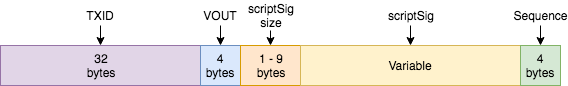
\includegraphics[scale=0.57]{img/Bitcoin_transactions_data_input.png}
        \caption{Los 5 segmentos de datos en una entrada o \textit{input}.}
    \end{figure}
    
    \subsubsection{TXID}
    
    \begin{figure}[H]
        \texttt{0x0100000001\colorbox{Yellow}{000000000000000000000000000000000000000000000}} \\
        \texttt{\colorbox{Yellow}{0000000000000000000}ffffffff6003636004062f503253482f04358b} \\
        \texttt{0553084404f253000017e446522cfabe6d6d690688fb886c0df0c87cb} \\
        \texttt{c7ea4f7f1b5c0050bd0ac3751cfc997d9d6971328de04000000000000} \\
        \texttt{004861707079204e592120596f7572732047486173682e494f0000000} \\
        \texttt{001cb813195000000001976a91480ad90d403581fa3bf46086a91b2d9} \\
        \texttt{d4125db6c188ac00000000}
    \end{figure}
    
    Se trata del un \textit{hash} de 32 \textit{bytes} que representa la transacción que contiene la salida o el \textit{output} que se va a gastar en esta transacción. Una de las características que diferencia a una transacción de tipo \textit{Coinbase} del resto es que el valor de TXID es un numero hexadecimal con valor cero.
    \begin{figure}[H]
        \texttt{0x0000000000000000000000000000000} \\
        \texttt{000000000000000000000000000000000}
    \end{figure}
    En una transacción corriente este dato se obtiene aplicando la función hash SHA-256 dos veces a los datos de la transacción en formato \textit{Little-Endian}.
    
    \subsubsection{VOUT}
    
    \begin{figure}[H]
        \texttt{0x0100000001000000000000000000000000000000000000000000000} \\
        \texttt{0000000000000000000\colorbox{Yellow}{ffffffff}6003636004062f503253482f04358b} \\
        \texttt{0553084404f253000017e446522cfabe6d6d690688fb886c0df0c87cb} \\
        \texttt{c7ea4f7f1b5c0050bd0ac3751cfc997d9d6971328de04000000000000} \\
        \texttt{004861707079204e592120596f7572732047486173682e494f0000000} \\
        \texttt{001cb813195000000001976a91480ad90d403581fa3bf46086a91b2d9} \\
        \texttt{d4125db6c188ac00000000}
    \end{figure}
    
    En Bitcoin todas las salidas u \textit{outputs} de una transacción se almacenan en un dato de tipo vector. VOUT es un número hexadecimal con una longitud de 4 \textit{bytes} que representa el índice de las salidas u \textit{outputs} de una transacción en dicho vector. Otra de las características de una transacción de tipo \textit{Coinbase} es que el valor para VOUT es siempre \texttt{0xffffffff}, el número de 4 \textit{bytes} de más alto valor.
    \begin{figure}[H]
        \texttt{0xffffffff}
    \end{figure}
    
    \subsubsection{scriptSig size}
    
    \begin{figure}[H]
        \texttt{0x0100000001000000000000000000000000000000000000000000000} \\
        \texttt{0000000000000000000ffffffff\colorbox{Yellow}{60}03636004062f503253482f04358b} \\
        \texttt{0553084404f253000017e446522cfabe6d6d690688fb886c0df0c87cb} \\
        \texttt{c7ea4f7f1b5c0050bd0ac3751cfc997d9d6971328de04000000000000} \\
        \texttt{004861707079204e592120596f7572732047486173682e494f0000000} \\
        \texttt{001cb813195000000001976a91480ad90d403581fa3bf46086a91b2d9} \\
        \texttt{d4125db6c188ac00000000}
    \end{figure}
    
    Esta variable es un tiene por valor un número hexadecimal de longitud variable, desde 1 hasta 9 \textit{bytes} que representa el tamaño en \textit{bytes} que tendrán los datos almacenados en \textit{scriptSig}.
    \begin{figure}[H]
        \texttt{0x60}
    \end{figure}
    En este caso el tamaño es de \texttt{0x60}, que tras convertirlo a base decimal son 96 \textit{bytes}. Para este dato existe límite de tamaño que actualmente es de 1650 \textit{bytes}.
    
    \subsubsection{scriptSig}
    
    \begin{figure}[H]
        \texttt{0x0100000001000000000000000000000000000000000000000000000} \\
        \texttt{0000000000000000000ffffffff60\colorbox{Yellow}{03636004062f503253482f04358b}} \\
        \texttt{\colorbox{Yellow}{0553084404f253000017e446522cfabe6d6d690688fb886c0df0c87cb}} \\
        \texttt{\colorbox{Yellow}{c7ea4f7f1b5c0050bd0ac3751cfc997d9d6971328de04000000000000}} \\
        \texttt{\colorbox{Yellow}{004861707079204e592120596f7572732047486173682e494f}0000000} \\
        \texttt{001cb813195000000001976a91480ad90d403581fa3bf46086a91b2d9} \\
        \texttt{d4125db6c188ac00000000}
    \end{figure}
    
    Cuando en una transacción se generan salidas u \textit{outputs}, estas salidas se establecen con un \textit{script} de bloqueo, por lo tanto para poder utilizarlas como entradas o \textit{inputs} en las nuevas transacciones antes se debe debe utilizar un \textit{script} de desbloqueo llamado \textit{scriptSig}. Se trata de un dato de de longitud variable, en este caso tiene una longitud de 96 \textit{bytes} pero podría contener más o menos información, dependiendo de las operaciones que se quieran realizar en el \textit{script} o el mensaje que se quiera incluir. Adicionalmente lo utilizan los mineros para incluir mensajes de texto personalizados empleando caracteres ASCII, normalmente el nombre del minero o del pool de minería que ha resuelto el hash válido para poder minar el bloque. En este caso la transacción \textit{Coinbase} contiene el siguiente valor para el segmento de datos \textit{scriptSig}.
    \begin{figure}[H]
        \texttt{0x03636004062f503253482f04358b0553084404f253000017e446522c} \\
        \texttt{fabe6d6d690688fb886c0df0c87cbc7ea4f7f1b5c0050bd0ac3751cfc9}
        \texttt{97d9d6971328de04000000000000004861707079204e592120596f7572}
        \texttt{732047486173682e494f}
        
    \end{figure}
    
    En una representación de carácteres ASCII se vería de la siguiente forma:
    \begin{figure}[H]
    \centering
        \texttt{`.c`../P2SH/.5..S.D..S....FR,..mmi....l...|.\textasciicircum....}
        \texttt{......7Q.......(.........Happy NY! Yours GHash.IO}
    \end{figure}
    
    Realmente esta cadena de 96 \textit{bytes} es un \textit{script} o programa con una secuencia de instrucciones ordenadas en lenguaje \textit{Bitcoin Script} o simplemente \textit{script}. En la siguiente muestra se pueden ver los diferentes segmentos en los que se divide la cadena hexadecimal de \textit{scriptSig} en el caso concreto de esta transacción de tipo \textit{Coinbase} de ejemplo.
    
    \begin{figure}[H]
        $\begin{array}{lcl}
            \texttt{0x03} & \Rightarrow & \textbf{\texttt{OP\_PUSHBYTES\_3}} \\
            \texttt{0x636004} & \Rightarrow & \texttt{0x636004}\\
            \texttt{0x06} & \Rightarrow & \textbf{\texttt{OP\_PUSHBYTES\_6}} \\
            \texttt{0x2f503253482f} & \Rightarrow & \texttt{0x2f503253482f} \\
            \texttt{0x04} & \Rightarrow & \textbf{\texttt{OP\_PUSHBYTES\_4}} \\
            \texttt{0x358b0553} & \Rightarrow & \texttt{0x358b0553} \\
            \texttt{0x08} & \Rightarrow & \textbf{\texttt{OP\_PUSHBYTES\_8}} \\
            \texttt{0x4404f253000017e4} & \Rightarrow & \texttt{0x4404f253000017e4} \\
            \texttt{0x46} & \Rightarrow & \textbf{\texttt{OP\_PUSHBYTES\_70}} \\
            \texttt{0x522cfabe6d6d690688fb886c} & & \texttt{0x522cfabe6d6d690688fb886c} \\
            \texttt{0df0c87cbc7ea4f7f1b5c0050b} & & \texttt{0df0c87cbc7ea4f7f1b5c0050b} \\
            \texttt{d0ac3751cfc997d9d6971328de} & \Rightarrow & \texttt{d0ac3751cfc997d9d6971328de} \\
            \texttt{04000000000000004861707079} & & \texttt{04000000000000004861707079} \\
            \texttt{204e592120596f757273204748} & & \texttt{204e592120596f757273204748} \\
            \texttt{6173682e494f} & & \texttt{6173682e494f}
        \end{array}$
    \end{figure}
    
    Este \textit{script} introducirá diferentes datos en una pila que inicialmente está vacía. Para evitar que varias transacciones de tipo \textit{Coinbase} pertenecientes a diferentes bloques tengan el mismo valor en TXID se decidió implementar mediante la propuesta BIP34\footnote{https://github.com/bitcoin/bips/blob/master/bip-0034.mediawiki} un sistema que añade al inicio del \textit{script} un bloque de 4 \textit{bytes}, dividido en las siguientes dos secciones:
    
    \begin{itemize}
    \item La primera es una constante\footnote{https://en.bitcoin.it/wiki/Script\#Constants} de 1 \textit{byte} de longitud que representa un OP\_CODE, en este caso con valor \texttt{0x03}, e indica que el siguiente dato que se va a colocar en la pila tiene una longitud de 3 \textit{bytes}. Para ello se utiliza el OP\_CODE \textbf{\texttt{OP\_PUSHBYTES\_3}}.
    \item La segunda sección es un dato de 3 \textit{bytes} en formato \textit{Little-Endian} que representan la altura o el número del bloque al que pertenece la transacción \textit{Coinbase}, en este caso \texttt{0x636004}. La transacción \textit{Coinbase} que se ha utilizado en este ejemplo pertenece al bloque número \texttt{\#}286819 de la cadena de bloques de \textit{Bitcoin} en la red principal \textit{mainnet}. Si se convierten los 3 \textit{bytes} \texttt{0x636004} a formato \textit{Big-Endian} se obtiene el valor hexadecimal \texttt{0x046063}, que en base 10 o decimal es el número 286819 y se corresponde con el número de bloque al que pertenece esta transacción.
    \end{itemize}
    
    \begin{minipage}{0.45\textwidth}
        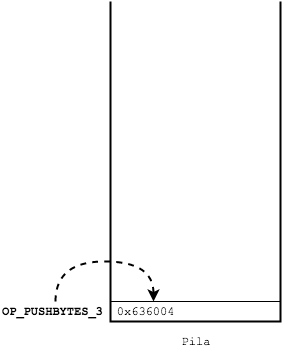
\includegraphics[scale=0.57]{img/Bitcoin_transactions_stack_01.png}
    \end{minipage}
    \hfill
    \begin{minipage}{0.45\textwidth}
        Así pues, mediante la instrucción \textbf{\texttt{OP\_PUSHBYTES\_3}} se añaden los siguientes 3 \textit{bytes} a la pila.
    \end{minipage}
    
    
    
    \subsubsection{Sequence}
    
    \begin{figure}[H]
        \texttt{0x0100000001000000000000000000000000000000000000000000000} \\
        \texttt{0000000000000000000ffffffff6003636004062f503253482f04358b} \\
        \texttt{0553084404f253000017e446522cfabe6d6d690688fb886c0df0c87cb} \\
        \texttt{c7ea4f7f1b5c0050bd0ac3751cfc997d9d6971328de04000000000000} \\
        \texttt{004861707079204e592120596f7572732047486173682e494f\colorbox{Yellow}{0000000}} \\
        \texttt{\colorbox{Yellow}{0}01cb813195000000001976a91480ad90d403581fa3bf46086a91b2d9} \\
        \texttt{d4125db6c188ac00000000}
    \end{figure}
    
    Se trata de un número de 4 \textit{bytes} de longitud, se utiliza para permitir que las transacciones no confirmadas que tengan un \textit{Locktime} se actualicen antes de darlas por finalizadas o confirmadas. También se utiliza para desactivar el \textit{Locktime} de la transacción. En el caso de una transacción de tipo \textit{Coinbase} se establece este valor a cero.
    \begin{figure}[H]
        \texttt{0x00000000}
    \end{figure}
    Se implementó en el año 2015 mediante la propuesta BIP125\footnote{https://github.com/bitcoin/bips/blob/master/bip-0125.mediawiki}, hasta entonces no se le daba uso.
    
    \subsection{Output}
    
    \begin{figure}[H]
        \texttt{0x0100000001000000000000000000000000000000000000000000000} \\
        \texttt{0000000000000000000ffffffff6003636004062f503253482f04358b} \\
        \texttt{0553084404f253000017e446522cfabe6d6d690688fb886c0df0c87cb} \\
        \texttt{c7ea4f7f1b5c0050bd0ac3751cfc997d9d6971328de04000000000000} \\
        \texttt{004861707079204e592120596f7572732047486173682e494f0000000} \\
        \texttt{0\colorbox{Yellow}{01cb813195000000001976a91480ad90d403581fa3bf46086a91b2d9}} \\
        \texttt{\colorbox{Yellow}{d4125db6c188ac00000000}}
    \end{figure}
    
    En una transacción hay un segmento de datos para las salidas u \textit{outputs} y este a su vez se divide en los siguientes cinco segmentos:
    
    \begin{itemize}
    \item Output count
    \item Output value
    \item scriptPubKey size
    \item scriptPubKey
    \item Locktime
    \end{itemize}
    
    \begin{figure}[H]
    \centering
        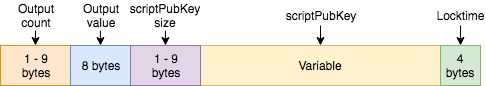
\includegraphics[scale=0.57]{img/Bitcoin_transactions_data_output.png}
        \caption{Los 5 segmentos de datos en una salida u \textit{output}.}
    \end{figure}
    
    \subsubsection{Output count}
    
    \begin{figure}[H]
        \texttt{0x0100000001000000000000000000000000000000000000000000000} \\
        \texttt{0000000000000000000ffffffff6003636004062f503253482f04358b} \\
        \texttt{0553084404f253000017e446522cfabe6d6d690688fb886c0df0c87cb} \\
        \texttt{c7ea4f7f1b5c0050bd0ac3751cfc997d9d6971328de04000000000000} \\
        \texttt{004861707079204e592120596f7572732047486173682e494f0000000} \\
        \texttt{0\colorbox{Yellow}{01}cb813195000000001976a91480ad90d403581fa3bf46086a91b2d9} \\
        \texttt{d4125db6c188ac00000000}
    \end{figure}
    
    Esta variable es un tiene por valor un número entero positivo de longitud variable, desde 1 hasta 9 \textit{bytes}, y representa el número de salidas u \textit{outputs} que tiene la transacción.
    \begin{figure}[H]
        \texttt{0x01}
    \end{figure}
    
    \subsubsection{Output (Value)}
    
    \begin{figure}[H]
        \texttt{0x0100000001000000000000000000000000000000000000000000000} \\
        \texttt{0000000000000000000ffffffff6003636004062f503253482f04358b} \\
        \texttt{0553084404f253000017e446522cfabe6d6d690688fb886c0df0c87cb} \\
        \texttt{c7ea4f7f1b5c0050bd0ac3751cfc997d9d6971328de04000000000000} \\
        \texttt{004861707079204e592120596f7572732047486173682e494f0000000} \\
        \texttt{001\colorbox{Yellow}{cb81319500000000}1976a91480ad90d403581fa3bf46086a91b2d9} \\
        \texttt{d4125db6c188ac00000000}
    \end{figure}
    
    Se trata de un número de 8 \textit{bytes} de longitud en formato \textit{Little-Endian} que representa la cantidad de satoshis\footnote{1 bitcoin = 100.000.000 satoshis} que podrán ser reclamados en futuras transacciones como \textit{input} para ser gastados de nuevo.
    \begin{figure}[H]
    \centering
        $\texttt{0x}\overbrace{\texttt{cb81319500000000}}^{Little-Endian} \Rightarrow \texttt{0x}\overbrace{\texttt{00000000953181cb}}^{Big-Endian} = 2503049675_{10}$
    \end{figure}
    
    En este caso 2503049675 \textit{satoshis} son 25.03049675 \textit{bitcoins} o BTC, y como es el \textit{output} de la transacción de tipo  es la recompensa que se llevará quien mine este bloque.
    
    \subsubsection{Output (scriptPubKey size)}
    
    \begin{figure}[H]
        \texttt{0x0100000001000000000000000000000000000000000000000000000} \\
        \texttt{0000000000000000000ffffffff6003636004062f503253482f04358b} \\
        \texttt{0553084404f253000017e446522cfabe6d6d690688fb886c0df0c87cb} \\
        \texttt{c7ea4f7f1b5c0050bd0ac3751cfc997d9d6971328de04000000000000} \\
        \texttt{004861707079204e592120596f7572732047486173682e494f0000000} \\
        \texttt{001cb81319500000000\colorbox{Yellow}{19}76a91480ad90d403581fa3bf46086a91b2d9} \\
        \texttt{d4125db6c188ac00000000}
    \end{figure}
    
    Esta variable es un tiene por valor un número hexadecimal de longitud variable, desde 1 hasta 9 \textit{bytes} que representa el tamaño en \textit{bytes} que tendrán los datos almacenados en \textit{scriptPubKey}.
    \begin{figure}[H]
        \texttt{0x19}
    \end{figure}
    En este caso el tamaño es de \texttt{0x19}, que tras convertirlo a base decimal son 25 \textit{bytes}.
    
    \subsubsection{Output (scriptPubKey)}
    
    \begin{figure}[H]
        \texttt{0x0100000001000000000000000000000000000000000000000000000} \\
        \texttt{0000000000000000000ffffffff6003636004062f503253482f04358b} \\
        \texttt{0553084404f253000017e446522cfabe6d6d690688fb886c0df0c87cb} \\
        \texttt{c7ea4f7f1b5c0050bd0ac3751cfc997d9d6971328de04000000000000} \\
        \texttt{004861707079204e592120596f7572732047486173682e494f0000000} \\
        \texttt{001cb8131950000000019\colorbox{Yellow}{76a91480ad90d403581fa3bf46086a91b2d9}} \\
        \texttt{\colorbox{Yellow}{d4125db6c188ac}00000000}
    \end{figure}
    
    Es un dato de longitud variable, en este caso de 25 \textit{bytes}, pero podría contener más o menos información. Se trata de un \textit{script} también llamado \textit{locking script} que implementa un mecanismo de bloqueo para un \textit{output} o salida, de modo que esta no pueda ser gastada hasta que no se desbloquee tras cumplirse una serie de condiciones, la mayoría de la veces ser el poseedor de la clave privada que puede desbloquear el \textit{script} en el que se utiliza una clave pública.
    
    \begin{figure}[H]
        \texttt{0x76a91480ad90d403581fa3bf46086a91b2d9d4125db6c188ac}
    \end{figure}
    
    Esta cadena de 25 \textit{bytes}, al igual que \textit{scriptSig} es una secuencia de instrucciones ordenadas en lenguaje \textit{Bitcoin Script} o simplemente \textit{script}. En la siguiente muestra se pueden ver los diferentes segmentos en los que se divide la cadena hexadecimal de \textit{scriptPubKey} en el caso concreto de esta transacción de tipo \textit{Coinbase} de ejemplo.
    
    \begin{figure}[H]
        $\begin{array}{lcl}
            \texttt{0x76} & \Rightarrow & \textbf{\texttt{OP\_DUP}} \\
            \texttt{0xa9} & \Rightarrow & \textbf{\texttt{OP\_HASH160}}\\
            \texttt{0x14} & \Rightarrow & \textbf{\texttt{OP\_PUSHBYTES\_20}} \\
            \texttt{0x80ad90d403581fa3bf4} & \Rightarrow & \texttt{0x80ad90d403581fa3bf4} \\
            \texttt{6086a91b2d9d4125db6c1} & & \texttt{6086a91b2d9d4125db6c1} \\
            \texttt{0x88} & \Rightarrow & \textbf{\texttt{OP\_EQUALVERIFY}} \\
            \texttt{0xac} & \Rightarrow & \textbf{\texttt{OP\_CHECKSIG}}
        \end{array}$
    \end{figure}
    En este escript se introducen 20 \textit{bytes} en la pila mediante el OP\_CODE \textbf{\texttt{OP\_PUSHBYTES\_20}}. Estos 20 \textit{bytes} se obtienen como resultado al realizar un cálculo en dos pasos. Véase en este ejemplo con la siguiente clave pública o \textit{pubKey} ficticia:
    
    \begin{figure}[H]
    \centering
        \scriptsize{publicKey: \texttt{0240e5c8ab050d1763201ea95707fa747d01c42df7db3e8e4784c0dcba027b4af0}}
    \end{figure}
    
    \begin{enumerate}
        \item Hay que aplicar la función \textit{hash} SHA-256 a la clave pública o \textit{pubKey}.
        \begin{figure}[H]
        \centering
            \scriptsize{$\underbrace{SHA256(\texttt{0240e5c8ab050d1763201ea95707fa747d01c42df7db3e8e4784c0dcba027b4af0})}$ \\
            \texttt{c12da6010de58147801cef8a508b1e3da7460002268751093c4e6aadcf0967a1}}
        \end{figure}
        
        \item Al resultado anterior hay que aplicarle la función \textit{hash} RIPEMD-160.
        \begin{figure}[H]
        \centering
            \scriptsize{$\underbrace{RIPEMD160(\texttt{c12da6010de58147801cef8a508b1e3da7460002268751093c4e6aadcf0967a1})}$ \\
            \texttt{6938581228f46c05efb6ad6f4497128f3c49f32a}}
        \end{figure}
    \end{enumerate}
    
    Este doble cálculo \textit{hash} se puede expresar mediante el siguiente resumen:
    
    \begin{figure}[H]
    \centering
        \scriptsize{\texttt{RIPEMD160(SHA256(pubKey)) = 6938581228f46c05efb6ad6f4497128f3c49f32a}}
    \end{figure}
    
    
    El resultado representa un dato que se utilizará más adelante para generar la dirección Bitcoin a la que se ha de enviar la cantidad de \textit{satoshis}. Pero antes es necesario añadir un byte de versión con valor \texttt{00} por la izquierda, 4 bytes de \textit{checksum} por la derecha\footnote{https://github.com/JavierDominguezGomez/Bitcoin\_cryptography/blob/master/tools/getCheckSum.sh} y aplicarle el esquema de codificación Base58\footnote{https://en.wikipedia.org/wiki/Base58} para obtener la dirección Bitcoin final.
    
    \subsubsection{Locktime}
    
    \begin{figure}[H]
        \texttt{0x0100000001000000000000000000000000000000000000000000000} \\
        \texttt{0000000000000000000ffffffff6003636004062f503253482f04358b} \\
        \texttt{0553084404f253000017e446522cfabe6d6d690688fb886c0df0c87cb} \\
        \texttt{c7ea4f7f1b5c0050bd0ac3751cfc997d9d6971328de04000000000000} \\
        \texttt{004861707079204e592120596f7572732047486173682e494f0000000} \\
        \texttt{001cb813195000000001976a91480ad90d403581fa3bf46086a91b2d9} \\
        \texttt{d4125db6c188ac\colorbox{Yellow}{00000000}}
    \end{figure}
    
    Se trata de un número de 4 \textit{bytes} de longitud en formato \textit{Little-Endian} que representa una medida de bloqueo para una transacción, es decir, una condición que mantiene bloqueada la transacción hasta que se cumpla la premisa. El valor  de ese consa premisa se establece mediante edicionalque tenga \textit{Locktime}, y ese valor puede hacer referencia bien a una altura de bloque o bien a una fecha en formato \textit{epoch} o \textit{unixtime}\footnote{https://es.wikipedia.org/wiki/Tiempo\_Unix}. Una vez se cumpla la fecha o la altura del bloque ya se podrá hacer uso de esa transacción. En el caso de una transacción de tipo \textit{Coinbase} no se establece ningún periodo de bloqueo.
    \begin{figure}[H]
        \texttt{0x00000000}
    \end{figure}
    
    La mayoría de las transacciones no utilizan el tiempo de bloqueo, por lo que suele establecer su valor a \texttt{0x00000000}. Por el contrario, se puede utilizar para asegurarse de que una transacción rmanecerápe bloqueada por un tiempo específico o hasta que no se llegue a una altura de bloque indicado.
    
\end{document}
